\section{Learning-Based Controller}
\label{sec:learning}

A learning-based controller is included to demonstrate that policies obtained
through reinforcement learning can be integrated into \mra{} without modifying
the race-management or evaluation framework. The controller receives the same
participant-side information available during normal benchmark operation, and its
gate progression and safety events are adjudicated by the independent referee
described in Section~\ref{sec:referee}.
Rather than treating learning as a separate benchmark mode, the policy is exposed
through the same controller interface used by the reference approaches.

The scope of this section is an integration demonstration: the recurrent PPO
controller shows that a learned policy can be integrated and evaluated through the
same participant-level information boundary, action interface and independent
referee. Training and evaluation both use the three official circuit families, so
the episodes reported in Section~\ref{sec:eval_rq5} describe behaviour on those
circuits and do not measure out-of-distribution generalization. No held-out course
geometry is involved, and none is claimed.

Fig.~\ref{fig:schematic_learning} summarizes the resulting control loop and the
training configuration.
\begin{figure}[t]
\centering
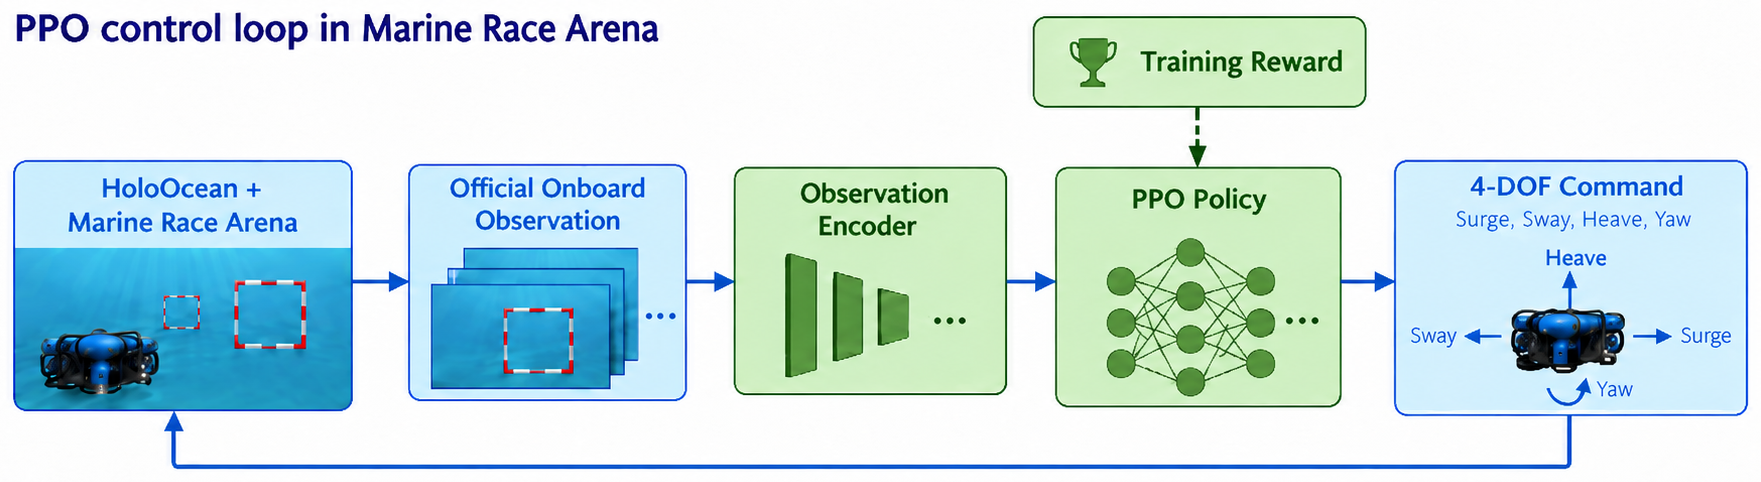
\includegraphics[width=\linewidth]{figures/p4_control_loop.png}
\caption{Control loop of the recurrent learning-based controller. The official
onboard observation is encoded and consumed by the policy, which returns the same
four-degree-of-freedom body-frame command as any other participant, while the
training reward acts only during training and never enters the observation.}
\label{fig:schematic_learning}
\end{figure}


\subsection{Observation Representation and Recurrent Policy}
\label{sec:learning_obs}

The policy receives a 27-dimensional observation vector built exclusively from
participant-accessible measurements. The representation combines acoustic
information associated with the locally tracked beacon, visual information about
the corresponding gate target, vehicle motion measurements and short-term
temporal information. It includes beacon availability, acoustic bearing,
elevation and range, visual target centre and apparent size, depth, body-frame
DVL velocity, yaw rate, the previous control action, short-term variations of the
visual and acoustic observations, an indicator of recent target transitions and,
when available, a local estimate of gate orientation. Availability indicators
are used to distinguish valid measurements from missing ones, while unavailable
quantities are represented through neutral values. Global vehicle pose, exact
gate coordinates, future course geometry and referee-derived progress are not
included.

The controller is trained with Proximal Policy Optimization
(PPO)~\cite{schulman2017ppo} using a recurrent actor--critic policy. The
implementation is the \texttt{RecurrentPPO} algorithm of sb3-contrib, the
contributed extension of Stable-Baselines3~\cite{raffin2021sb3}. The recurrent
component is implemented with LSTM memory, so the decision at the current control
step depends not only on the present observation but also on information retained
from the recent observation history. This is useful in gate racing because the
problem is only partially observable from a single frame: visual detections may
be incomplete or temporarily disappear close to the aperture, acoustic
measurements evolve continuously during the approach and the same instantaneous
observation may correspond to different phases of a passage depending on the
vehicle's recent motion.

At each step, the current observation is first mapped to an internal feature
representation and then processed together with the recurrent state maintained by
the LSTM. The resulting temporal representation is shared by the actor--critic
architecture: the actor produces the continuous control action, while the critic
estimates the state value used during PPO optimization. The recurrent state is
carried forward between consecutive control steps and reset at the beginning of a
new episode. In this way, temporal context is learned directly by the policy
instead of being supplied through an explicit handcrafted navigation state
machine.

\subsection{Released Training Campaign}
\label{sec:learning_training}

The released recurrent policy was fine-tuned from a preceding policy using
full-circuit episodes across the three official circuits. The campaign draws on
two alternating full-circuit copies per track, with no fragment or synthetic
source, and the released checkpoint records $50\,688$ training timesteps for this
final fine-tuning stage. The preceding policy it continues is identified in the
released campaign configuration; its own training budget is not part of that
figure. The observation representation and control interface are the ones
described above and are unchanged throughout.

The reward is defined over the same participant-level quantities. Successful gate
crossings and course completion provide the principal positive task signals, while
additional terms shape progress and alignment during the approach. Elapsed time,
collisions and terminal failures are penalized. These terms are used only to shape
the learning process and are not included in the observation seen by the
controller.

A single policy is selected on closed-loop completion over the official circuits
and frozen before the reported episodes, and the controller is then executed
without additional learning or online adaptation. The released checkpoint, its
provenance and the hyperparameter and reward configuration are available in the
repository. Attempts that produced no valid episode because of a simulator or
engine fault rather than controller behaviour are recorded as technical-invalid
and excluded from the evaluation under that rule; the reported PPO results
comprise nine valid evaluation episodes. The results of this fixed policy are
reported together with the other benchmark evaluations in
Section~\ref{sec:eval_rq5}.
